\section{Estruturas}

O foco do grupo de estruturas é elaborar e calcular toda a parte mecânica do projeto, bem como definir o sistema de bombeamento e arrefecimento. É de extrema importância para o projeto e para todos os subgrupos que, seja efetuada de maneira precisa a montagem da estrutura e da sua análise de risco e orçamento.

\subsection{Metodologia de trabalho}

Durante as pesquisas realizadas pelo grupo, constaram inúmeras hipóteses de montagem do sistema que estarão descritas ao longo do relatório. Com o objetivo de facilitar e agilizar as pesquisas realizadas, o grupo se subdividiu em 5 (cinco) subgrupos, sendo estes: projeto conceitual de bombeamento e arrefecimento, projeto conceitual de tubulações e conectores, projeto conceitual do líquido de arrefecimento, avaliação de riscos técnicos nos sistemas de bombeamento e arrefecimento e avaliação de riscos técnicos nas tubulações e conectores. 

\subsection{Estrutura do sistema}

A montagem geral da estrutura do projeto será baseada no esquemático da figura abaixo. Nele constam: 4 (quatro) coolers, um reservatório, duas válvulas de redirecionamento de fluxo, duas bombas e a tubulação (incluindo os conectores não ilustrados). O projeto consiste em bombear a água do reservatório para o sensor da Kistler, que aquecerá o líquido. Após o contato com o sensor, a água retorna ao sistema passando pelo radiador, onde será resfriada e adicionada de volta ao reservatório.

\begin{figure}[!htb]                                                               
   \centering                                                                      
   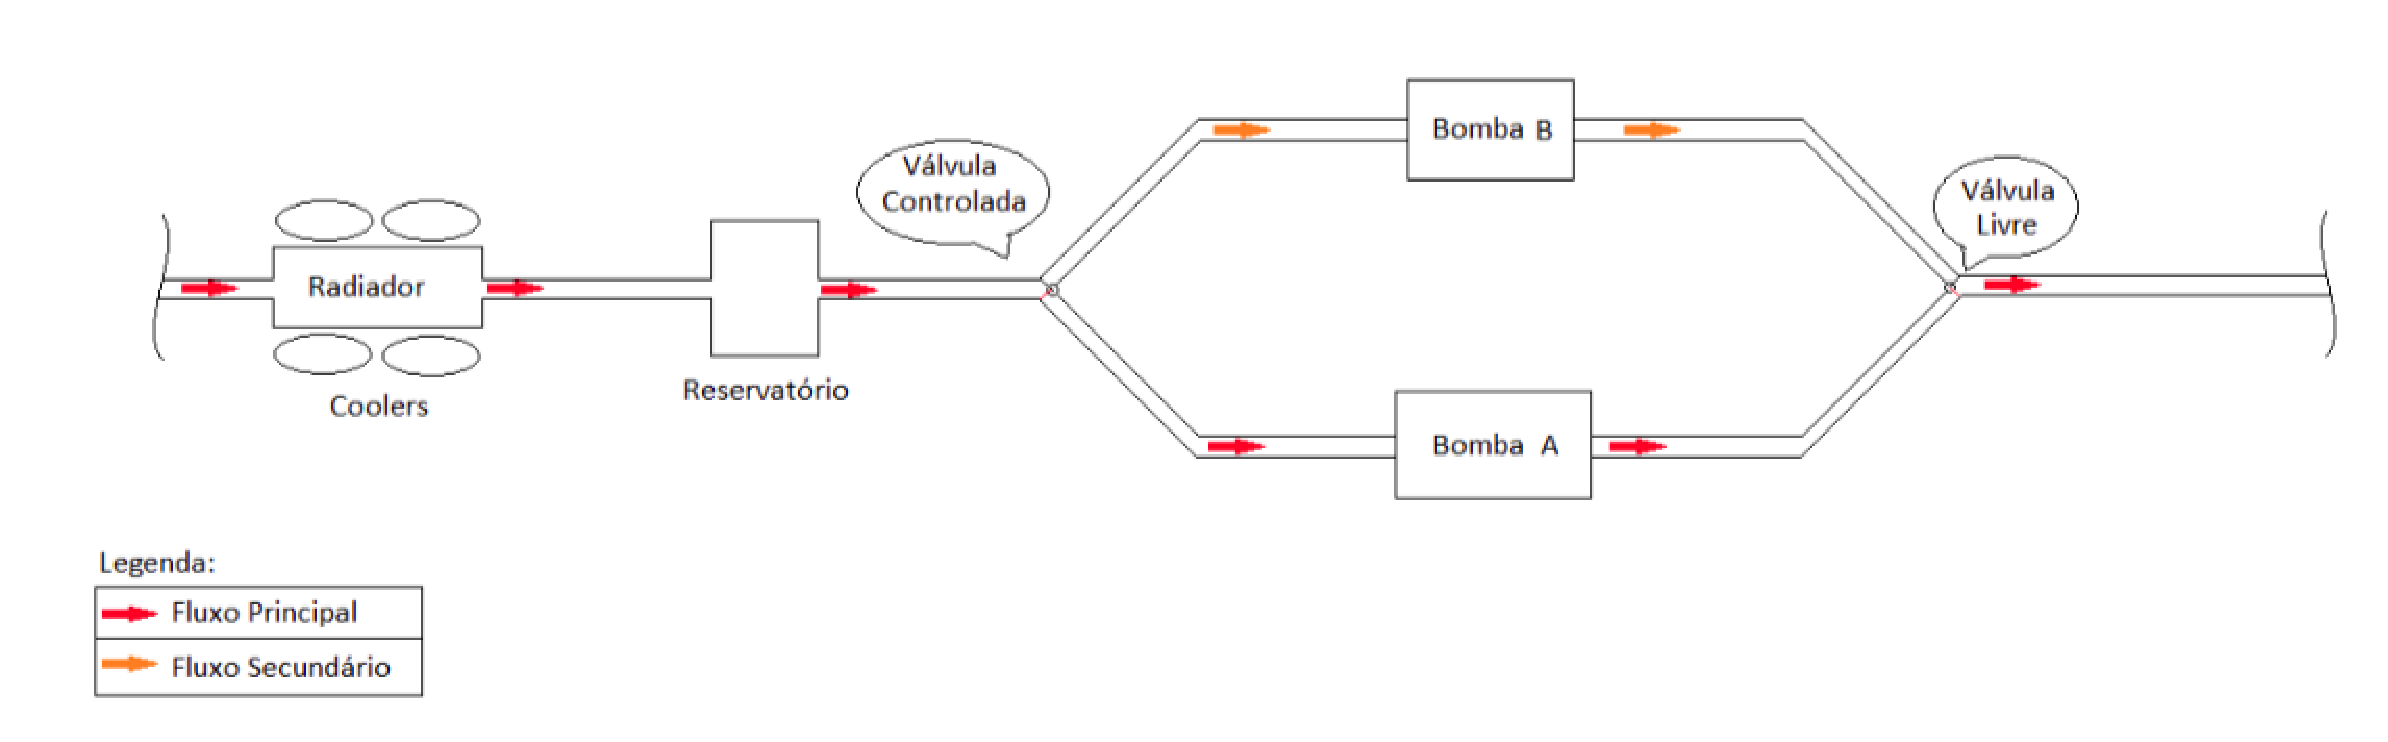
\includegraphics[width=15cm, keepaspectratio=true]{figuras/projetoestrutural.eps}
   \caption{Esquemático geral do projeto de estrutura}                        
\end{figure}


\subsection{Sistema de bombeamento e arrefecimento}

Como base para o projeto conceitual do sistema de arrefecimento e bombeamento utilizamos, conforme sugerido pelo professor (Anexo 1), o uso de um sistema de water cooling semelhante ao utilizado no resfriamento de processador para computadores. Partindo dessa premissa, foram avaliadas as seguintes possibilidades:

\begin{itemize}
\item Utilização de um watercooler comercial;
\item Montagem de um watercooler com peças avulsas.
\end{itemize}

Sobre o primeiro tópico, o uso de um watercooler comercial foi avaliado tendo em vista três modelos: um considerado de acesso, um intermediário e um top de linha. Já sobre o segundo tópico, teve-se em mente a obtenção do melhor custo-benefício, com objetivo de comparar com os watercoolers comerciais estudados previamente e com os dados obtidos do sistema de resfriamento proprietário da Kistler.

\subsection{Possibilidade 1: Watercooler comercial}

\subsubsection{Kit de Montagem Thermaltake Pacific Reef 240 Petg Diy LCS Blue CL-W120-CA12BU-A}

Esse condiz com o top de linha encontrado em solo brasileiro para o resfriamento de processadores em computadores domésticos. O mesmo possui especificações exemplares, principalmente no que se refere à bomba, superando o sistema de resfriamento da Kistler no que se diz respeito à pressão em cerca de 1 bar (aprox. 3,5 contra 2,5) [2][3].
Apesar da sua viabilidade técnica, logo foi constatada a sua inviabilidade econômica para o projeto, esse classificado com low budget, sendo o preço do kit é de R\$ 2225,76 (dois mil duzentos e vinte e cinco reais e setenta e seis centavos) [4].

\begin{figure}[!htb]                                                               
   \centering                                                                      
   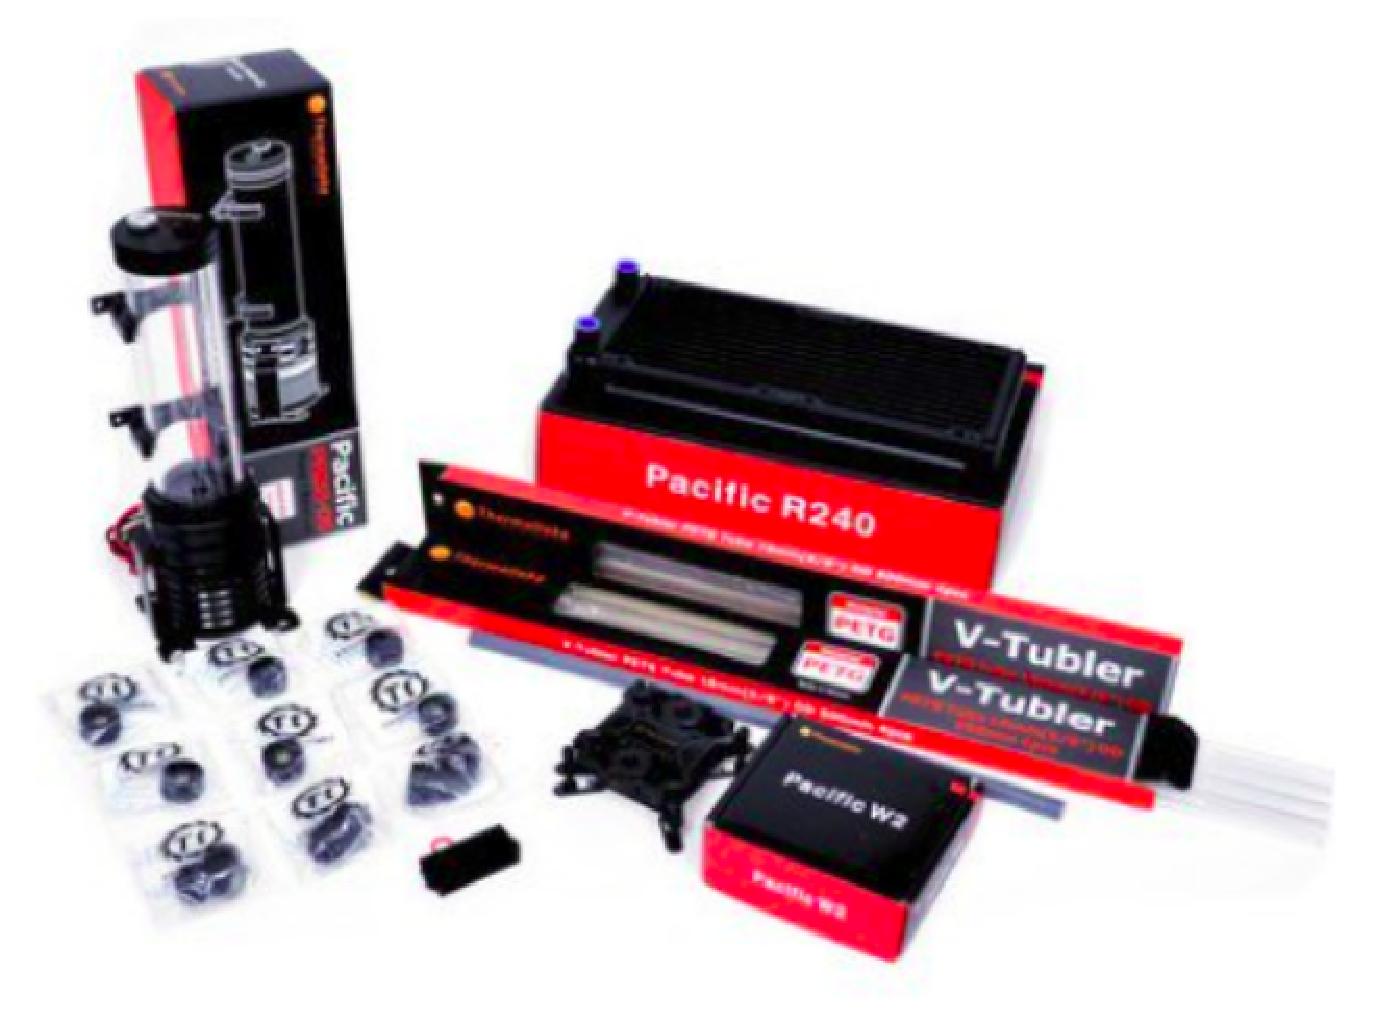
\includegraphics[scale=0.4, keepaspectratio=true]{figuras/watercooler1.eps}
   \caption{KIT DE MONTAGEM THERMALTAKE PACIFIC REEF 240 PETG DIY LCS BLUE CL-W120- CA12BU-A.}               
\end{figure}

\subsubsection{WaterCooler CoolerMaster Masterliquid Pro 240 MLY-D24M-A20MB-R1}

Agora referente aos modelos intermediários de mercado, há uma grande falta de informações, principalmente no que se refere as especificações mais técnicas de bomba e do radiador, fatores muito importantes para esse projeto. Sobre o radiador, nos foi informado apenas sobre o seu tamanho (275 x 118.5 x 27 mm) e o seu material (Alumínio). Sobre a bomba, apenas dados sobre nível de barulho, MTTF (Mean Time To Failure ou tempo médio para falhas), L-10 Life (tempo até primeira evidência de falhas) e voltagem de alimentação, dados esses que possuem a sua devida importância, porém, no que se refere ao fluxo de água no sensor e o seu resfriamento, são irrelevantes.
No entanto, os dados sobre as ventoinhas utilizadas são bem completos, sendo esse um dos componentes mais importantes no arrefecimento do líquido. Seus dados são os seguintes:

\begin{itemize}
\item Dimensões: 120 x 120 x 25 mm;
\item Velocidade: $650 ~ 2000 RPM (PWM) \pm 10$\%;
\item Fluxo de ar: 66,7 CFM (máx.);
\item Pressão de ar: 2,34 mmH2O (máx.);
\item MTTF: 490000 horas;
\item L-10 Life: 70000 horas;
\end{itemize}

Todos os dados foram obtidos da referência [5], a ficha do produto. Por causa disso, sua possibilidade de uso foi deixada em aberto, caso se visse a necessidade. Seu preço encontrado foi o de R\$ 670,47 (seiscentos e setenta reais e quarenta e sete centavos) [6].

\begin{figure}[!htb]                                                               
   \centering                                                                      
   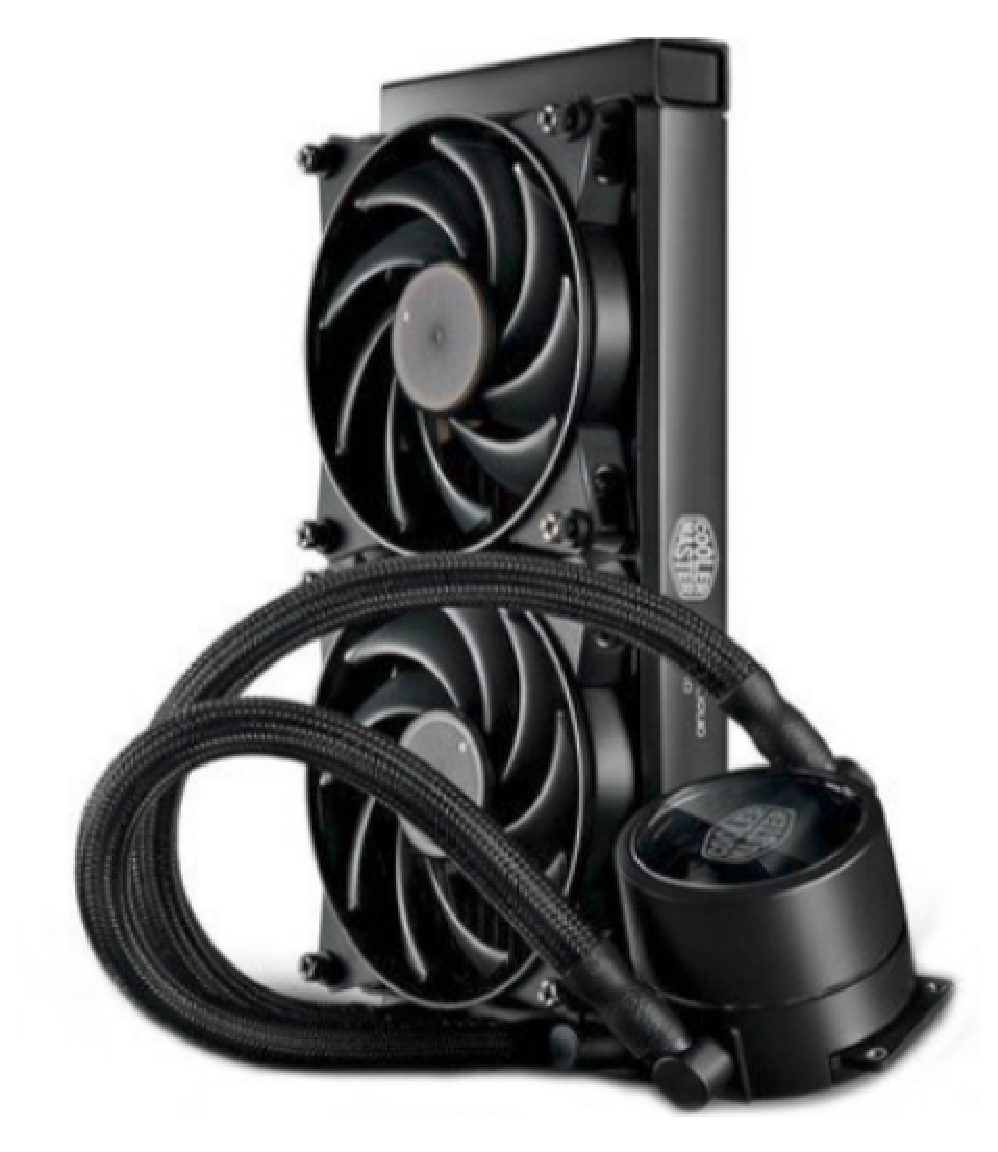
\includegraphics[scale=0.4, keepaspectratio=true]{figuras/watercooler2.eps}
   \caption{WATERCOOLER COOLERMASTER MASTERLIQUID PRO 240 MLY-D24M- A20MB-R1.}               
\end{figure}

\subsubsection{WaterCooler CoolerMaster 240V MLX-D24M-A20PW-R1}

Sobre os modelos de entrada encontrados no mercado brasileiro, o mesmo problema citado anteriormente persiste. Sobre o radiador possuímos os mesmos dados do anterior, tamanho (120 x 120 x 25 mm) e material (Alumínio). Sobre a bomba foram obtidos os mesmos dados encontrados anteriormente, com o acréscimo da dimensão da bomba. E novamente os dados sobre a ventoinha foram os mais completos, sendo os seguintes:
\begin{itemize}
\item Dimensões: 120 x 120 x 25 mm;
\item Velocidade: $650 - 2000 RPM (PWM) \pm 10$\%;
\item Fluxo de ar: 66.7 CFM (máx.);
\item Pressão de ar: $2.34 mmH2O \pm 10$\% (máx.);
\item MTTF: 160,000 hours;
\item L-10 Life: 22,800 hours.
\end{itemize}
Todos os dados foram obtidos da referência [7], a ficha técnica do produto. Dada as suas especificações técnicas observáveis semelhantes, a sua viabilidade se torna muito maior se comparando com o watercooler analisado anteriormente, principalmente por causa do seu preço médio R\$ 376,35 (trezentos e setenta e seis reais e trinta e cinco centavos) [8], praticamente a metade do encontrado anteriormente.

\begin{figure}[!htb]                                                               
   \centering                                                                      
   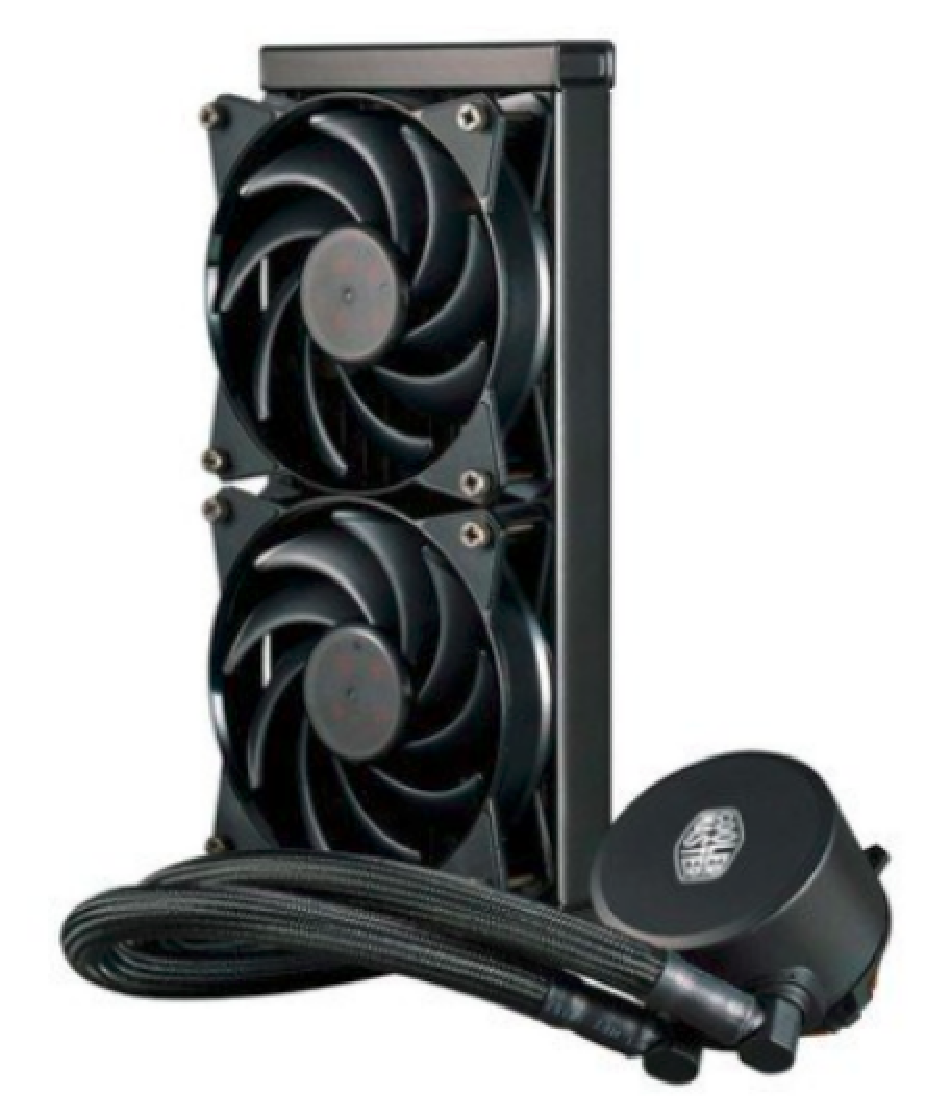
\includegraphics[scale=0.4, keepaspectratio=true]{figuras/watercooler3.eps}
   \caption{WATERCOOLER COOLERMASTER 240V MLX-D24M- A20PW-R1.}               
\end{figure}

\subsection{Possibilidade 2: Montagem do watercooler próprio}


Sobre isso, separou-se os componentes em três categorias: Bomba, radiador e ventoinha. A sua viabilidade técnica foi vista como foco o último watercooler analisado e o sistema de resfriamento proprietário da Kistler.

\subsubsection{Bomba}

O modelo da bomba escolhido foi o DC30QA-1230 [9] se encontra na referência [10], com suas especificações citadas abaixo:
\begin{itemize}
\item Vida útil: mais de 30000 horas;
\item Consumo: $DC12V / 350mA$;
\item Diâmetro externo de entrada e saída: 8,0 mm;
\item Fluxo máximo de água: $240L / H$;
\item Pressão de água: 3M (máx.);
\item Nível impermeável IP68
\item Temperatura máxima de operação: $60ºC$.
\end{itemize}

Sobre as especificações acima, é importante citar que o diâmetro de saída é o mesmo do sistema da Kistler e a bomba possui uma pressão máxima de 5 bar, mais de três vezes superior ao da Kistler, o que permite uma margem de trabalho. O seu preço é de U\$ 10,32 (dez dólares e trinta e dois centavos) [10].
 

\begin{figure}[!htb]                                                               
   \centering                                                                      
   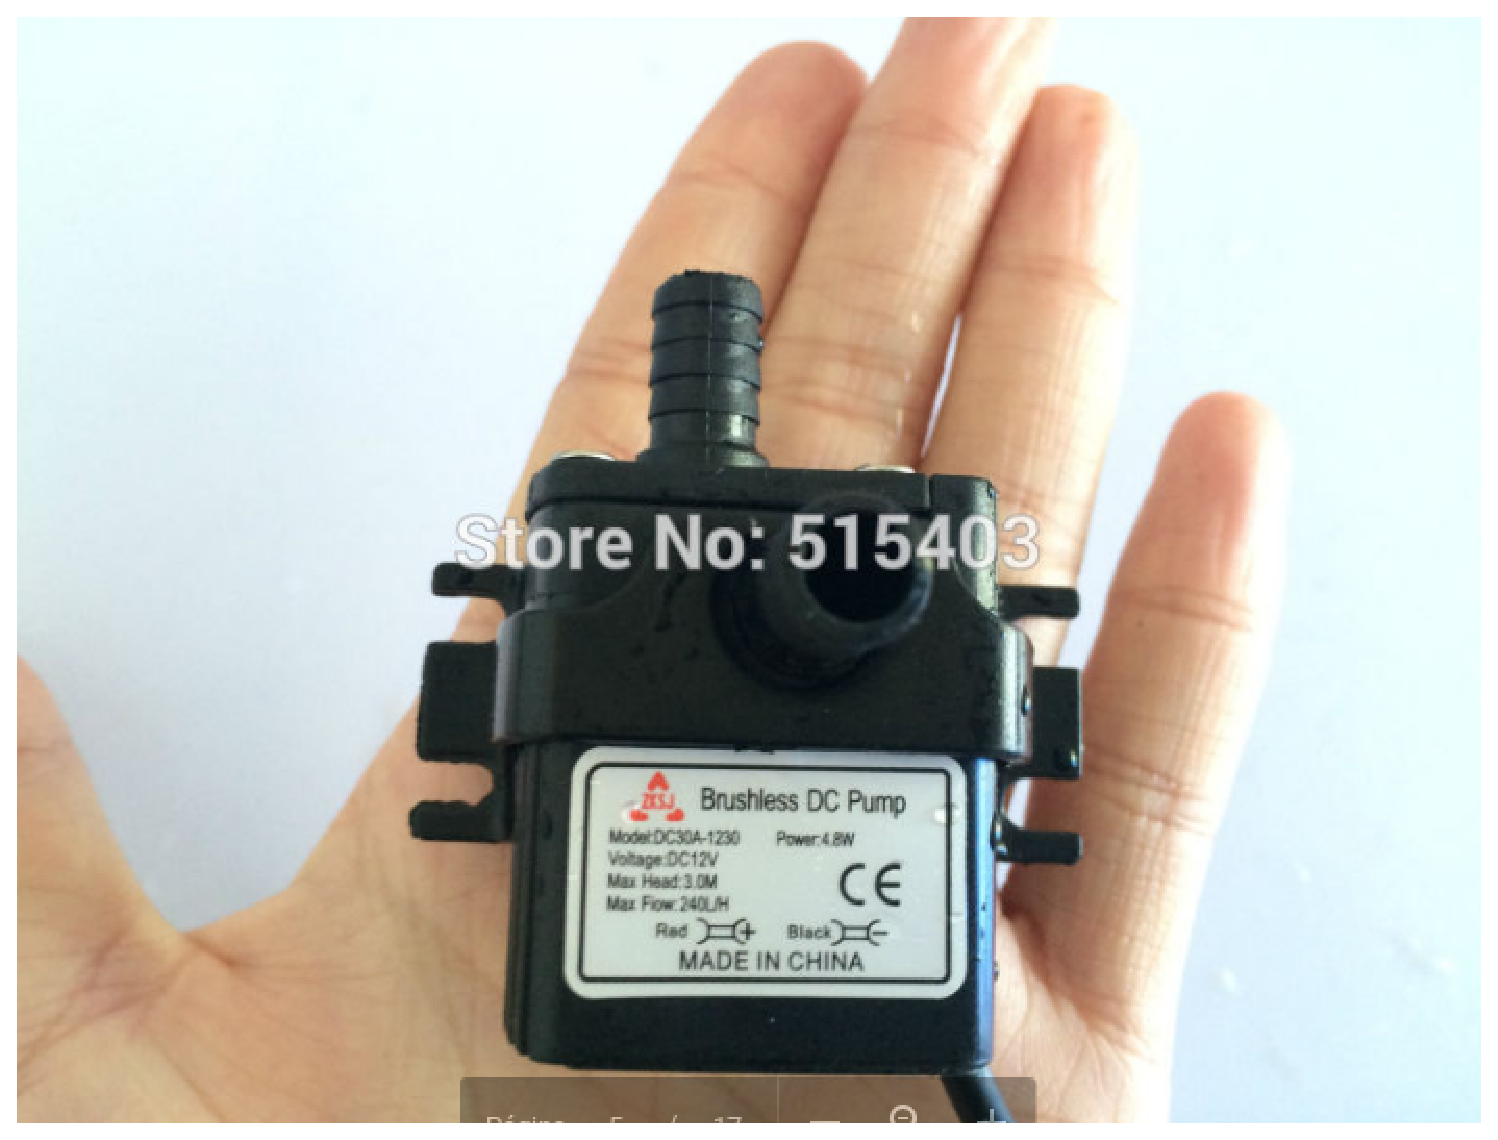
\includegraphics[scale=0.4, keepaspectratio=true]{figuras/bomba.eps}
   \caption{Bomba escolhida.}               
\end{figure}

\subsubsection{Radiador}

O modelo de radiador foi o mais difícil de se encontrar, devido à ausência de informações técnicas, tanto no que se refere ao sistema da Kistler, quanto no que se diz dos watercoolers. No entanto, conforme cita a referência [11], um site especializado em watercooler, assumindo radiadores do mesmo tamanho, o que fizemos ao longo das análises, escolhendo radiadores de 240 mm, a diferença de desempenho é muito pequena, sendo que fatores como a velocidade das ventoinhas tem influência muito maior do que a qualidade do radiador em si. Com isso em mente, escolhemos um radiador de alumínio com conexões G $1/4$, com preço de R\$ 150,00 (cento e cinquenta reais). [12]

\begin{figure}[!htb]                                                               
   \centering                                                                      
   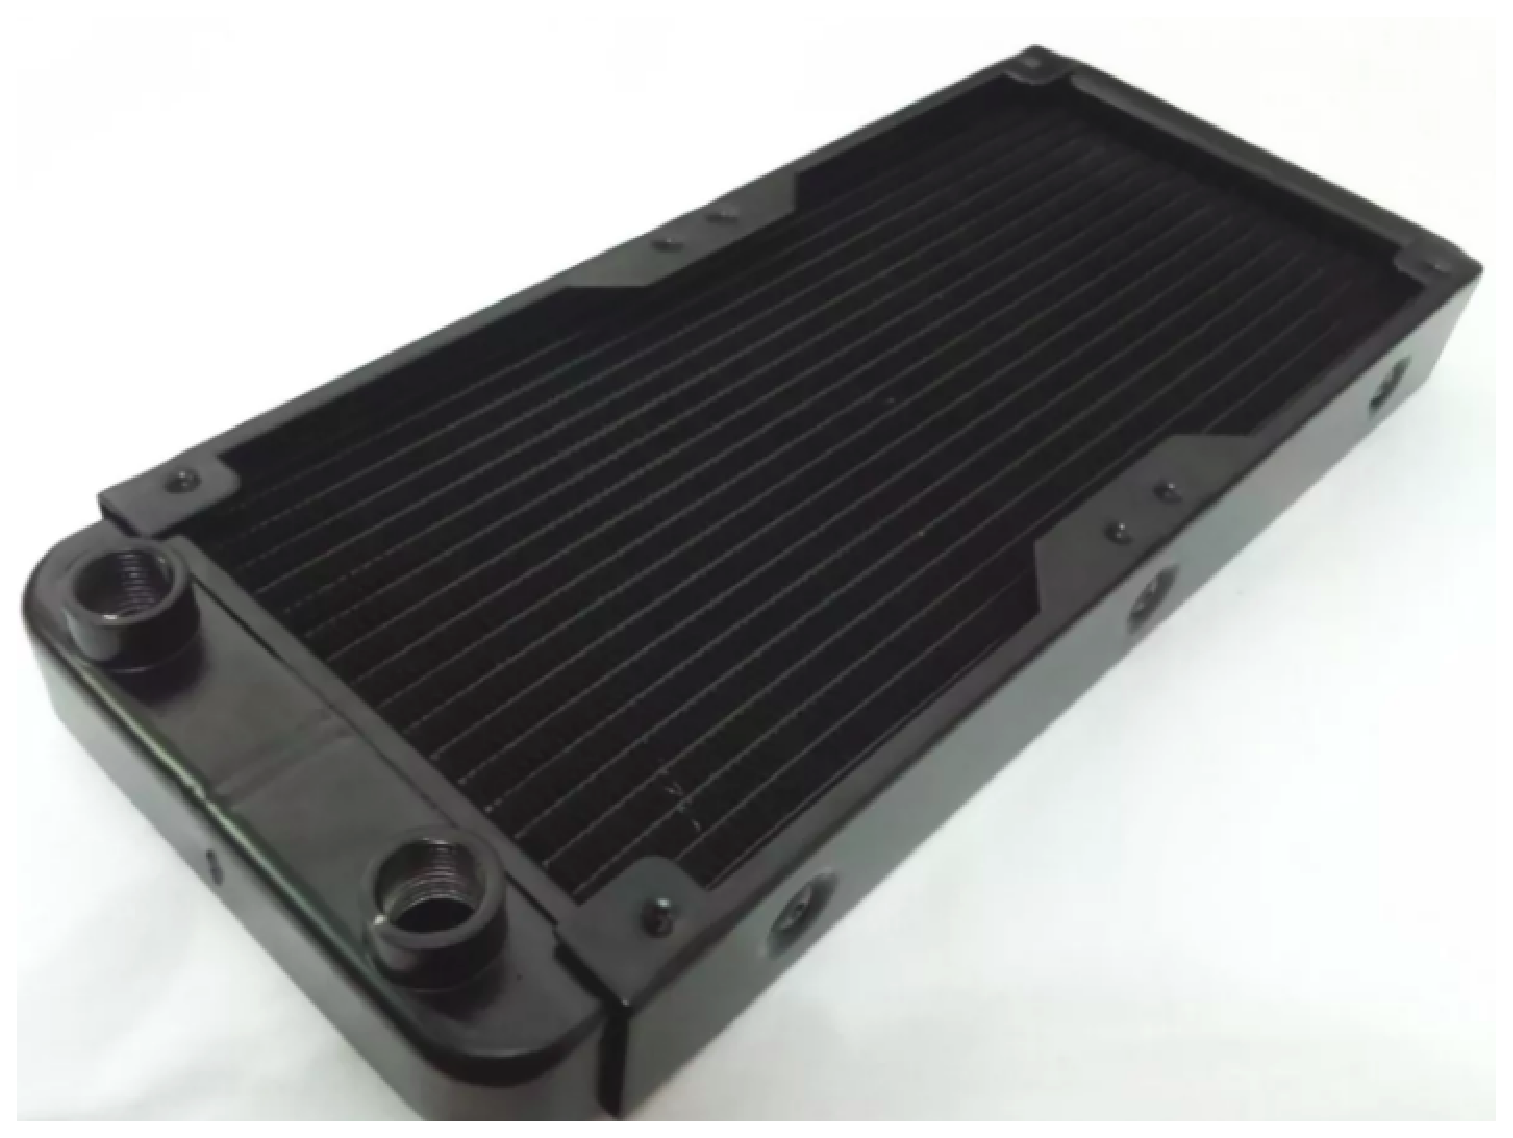
\includegraphics[scale=0.4, keepaspectratio=true]{figuras/radiador.eps}
   \caption{Radiador escolhido.}               
\end{figure}

\newpage
\subsubsection{Ventoinha}

Conforme citado anteriormente, as ventoinhas podem ser de uma maior importância que o próprio radiador, de forma que a escolha das mesmas foi feita buscando a melhor ventoinha possível a um custo-benefício adequado. Como parâmetro para a escolha da mesma, fora colocada as especificações técnicas da ventoinha analisada no watercooler de menor preço. 
Como resultado, a ventoinha escolhida foi a Cooler FAN “CoolerMaster Sickleflow 12cm R4-SXDP-20FB-R1 com LED Azul”, e suas especificações estão abaixo:

\begin{itemize}
\item Led Azul
\item Dimensões (A X L X P): 12,0 x 12,0 x 2,5 cmm
\item Velocidade: $2.000 RPM \pm 10$\%
\item Fluxo de ar: $69.69 CFM \pm 10$\%
\item Pressão de ar: $2.94 mmH2O \pm 10$\%
\item Expectativa de vida: 160,000 horas
\item Conector: 3 Pinos
\item Voltagem: 12VDC
\item Corrente: 0.35A
\item Consumo: 4.2W
\end{itemize}

A ventoinha escolhida possui uma velocidade de trabalho igual as do watercooler, mesma expectativa de vida útil, e mesmo tamanho. Porém, e mais importante, os fatores como fluxo de ar e pressão de ar encontrados são superiores a ventoinha do watercooler, o que foi considerado como ideal na escolha da mesma. Seu preço é de R\$ 35,18 (trinta e cinco reais e dezoito centavos) [13] e para o projeto serão necessárias quatro da mesma. Suas especificações técnicas foram encontradas na mesma referência que o seu preço.

\begin{figure}[!htb]                                                               
   \centering                                                                      
   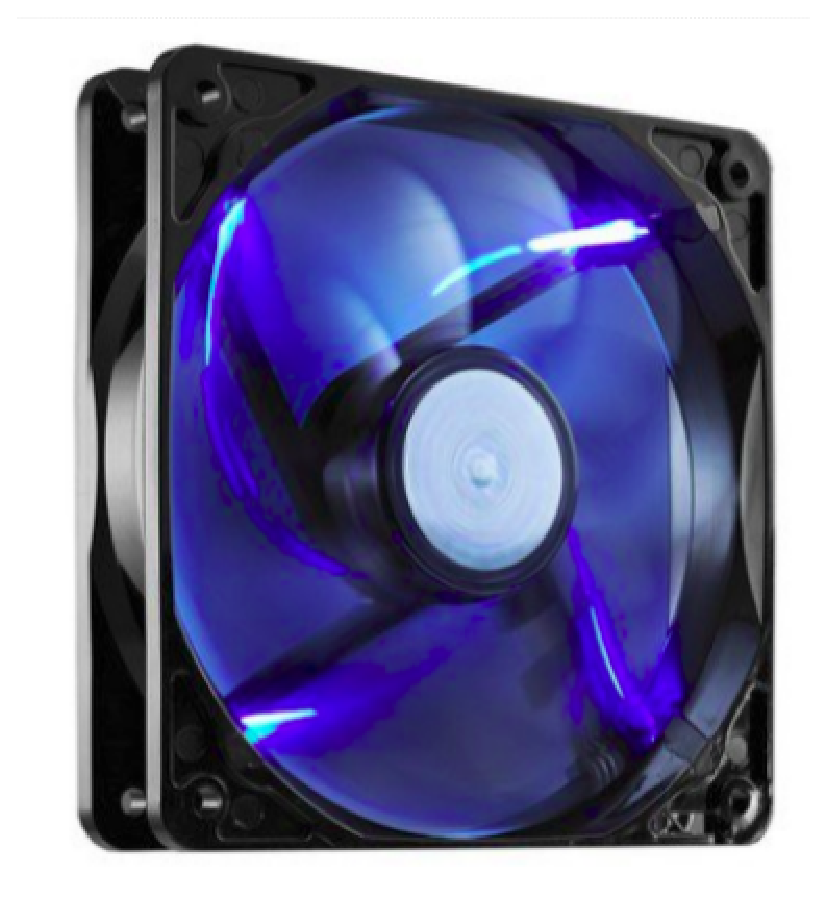
\includegraphics[scale=0.4, keepaspectratio=true]{figuras/ventoinha.eps}
   \caption{Ventoinha escolhida.}               
\end{figure}


\subsection{Líquido de arrefecimento}

O líquido de arrefecimento tem como função principal trocar calor com o sensor, refrigerando o sistema para evitar o sobreaquecimento.
Para isso o fluido de arrefecimento percorre a tubulação do sistema sem entrar em contato direto com os componentes eletrônicos do sensor, assim ele é resfriado graças à troca de calor entre a água (temperatura ambiente) e o sensor estimado em no máximo 450ºC.  Para que haja um fluxo controlado de água, será usado um sistema de bombeamento, garantindo a troca efetiva de calor.
O líquido de arrefecimento será a água pois, além de ser um fluido de fácil obtenção, possui propriedades térmicas e viscosas compatíveis com os requisitos do projeto a ser desenvolvido.
Sua capacidade térmica é bem elevada quando comparada com outras substâncias conhecidas (aproximadamente 1cal/g.ºC), além de possuir uma viscosidade baixa como é possível observar na tabela abaixo.

\newpage

\begin{figure}[!htb]                                                               
   \centering                                                                      
   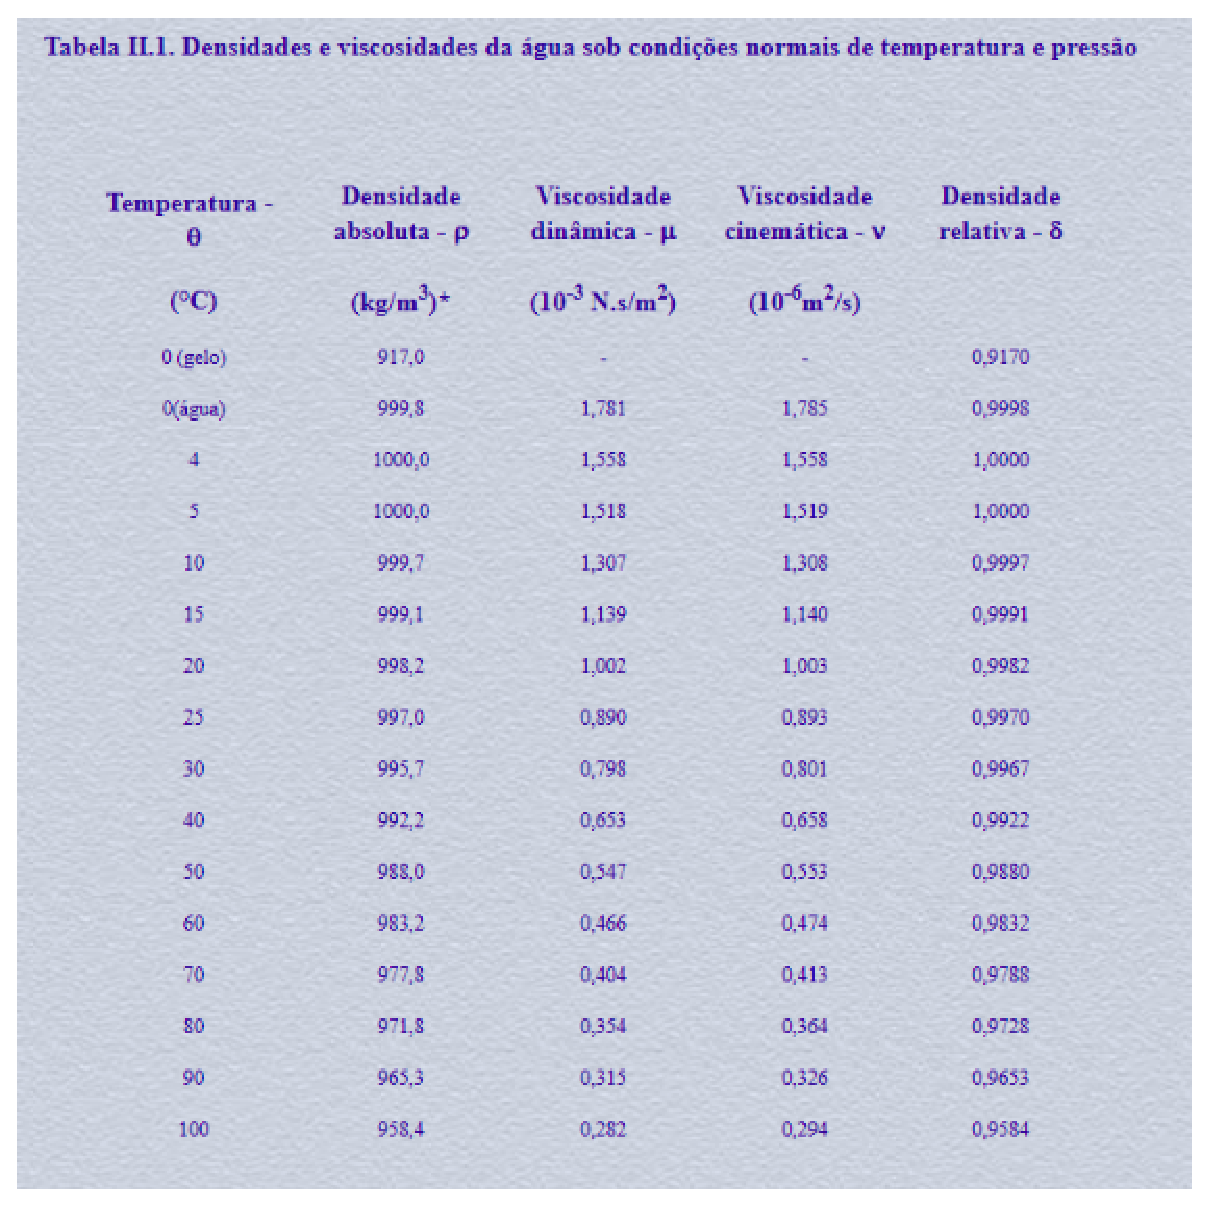
\includegraphics[scale=0.8, keepaspectratio=true]{figuras/tabelaagua.eps}               
\end{figure}

A água é um liquido em abundância e que pode ser facilmente encontrado. O litro de aguá mineral, que possui poucas impurezas, é cerca de um real e, a água destilada pode ser encontrada a R\$1,95 o litro [3]. Portanto, é um líquido de arrefecimento com pontos econômicos muito positivos.

\subsection{Tubulação}

\subsubsection{Tamanho}
É necessário um correto dimensionamento da sala onde se encontra o equipamento, ou seja:
\begin{itemize}
\item Posição do sensor na bancada de teste (Conhecido);
\item Posição do sistema de arrefecimento (Conhecido – 3 Opções)
\end{itemize}

\subsubsection{Material}
O material escolhido para a tubulação é o politetrafluoretileno (PTFE), família dos fluoroplásticos (PTFE, FEP, PFA, CTFE, ECTFE, ETFE, PVDF), que são resinas termoplásticas de estrutura principal parafínica que têm alguns ou todos os seus hidrogênios substituídos por átomos de flúor (C2F4)n. Caracteriza-se por excelentes propriedades dielétricas e resistência química, baixo coeficiente de atrito e excepcional estabilidade em elevadas temperaturas, resistência mecânica baixa ou moderada, custo elevado. 
O material foi escolhido por possuir excelentes propriedades, que são indispensáveis para o transporte do fluido de arrefecimento, bem como por contar com boa margem de segurança, já que todas as propriedades do material são superiores às necessitadas no projeto.

\begin{itemize}
\item Temperatura de trabalho: Possuem uma das mais amplas faixas de temperatura de trabalho, desde $-90ºC$ até $+240ºC$, em regime contínuo. A melhor opção em mangueiras para trabalho com vapor superaquecido.
\item Deslizamento sem atrito: Com baixo coeficiente de atrito, são particularmente indicados em sistemas mecânicos que apresentam dificuldade de lubrificação periódica.
\item Resistência à água e intempéries: São altamente hidrorrepelentes, apresentando absorção de umidade praticamente nula. Resiste aos raios solares, variações de umidade relativa do ar e da temperatura ambiente. 
\item Baixa aderência: Por ser antiaderente, o PTFE é o polímero adequado para tubos e mangueiras que conduzem líquidos viscosos e adesivos. 
\end{itemize}

\begin{figure}[!htb]                                                               
   \centering                                                                      
   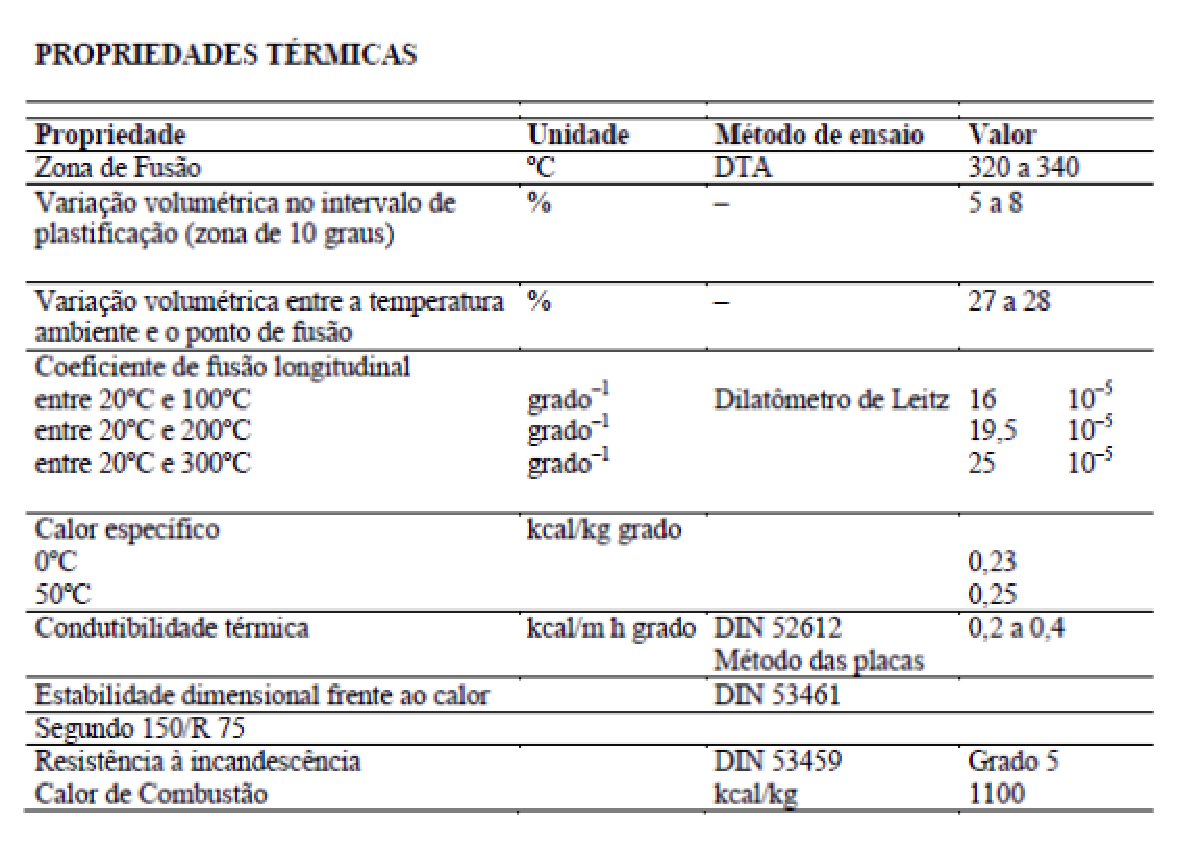
\includegraphics[scale=0.6, keepaspectratio=true]{figuras/tabela2.eps} 
   \caption{Dados fornecidos pela HOESCHT}              
\end{figure}

\subsubsection{Conectores}

Os conectores são importantíssimos para a correta montagem da tubulação, por serem conhecidos como os elos fracos na montagem da mesma, o grupo analisou e concordou com a utilização de conectores com melhor qualidade, mesmo tendo um custo mais alto, que se justifica pela vida útil e margem de segurança que os mesmos trazem ao sistema.
Os conectores escolhidos são da marca Swagelok, uma multinacional americana com mais de 50 anos de produção em conectores. Esses conectores possuem um tipo de travagem que fornece:
\begin{itemize}
\item Excelente vedação para gás e ação de crimpagem no tubo;
\item Fácil realização de corretas instalações;
\item Reapertos consistentes; 
\item Excelente resistência à fadiga por vibrações e suporte do tubo, etc.;
\end{itemize}

\begin{figure}[!htb]                                                               
   \centering                                                                      
   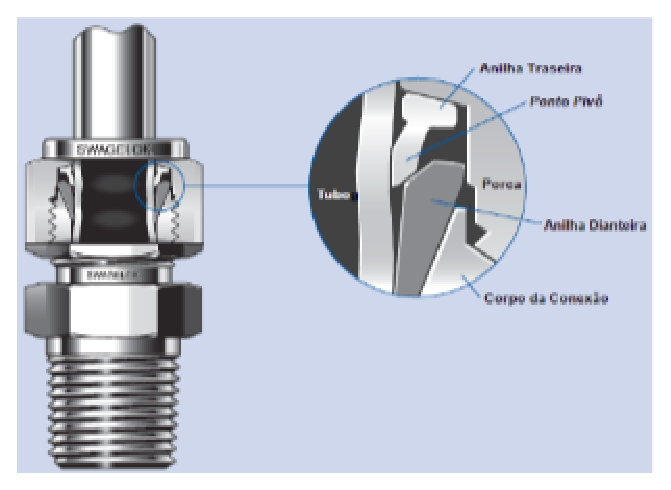
\includegraphics[scale=0.6, keepaspectratio=true]{figuras/conectores.eps} 
   \caption{Projeto de travagem dos conectores SWAGELOK.}              
\end{figure}

Como colocado acima a utilização dos mesmos é explicada por terem melhor resistência a: 

\begin{itemize}
\item Vazamentos
\item Vibração(cravamento no tubo)
\item Choque térmico
\item Corrosão
\end{itemize}

A Swagelok produz os conectores a partir dos mais diversos materiais, referente contato com a parte técnica da empresa foi conseguido documentos técnicos sobre valores máximos para temperatura e pressão, bem como o custo dos conectores de cada tipo de material, com isso pode-se realizar a correta escolha dos conectores para a utilização.
O material escolhido é o latão, seguindo o conselho do responsável técnico da Swagelok.

\begin{figure}[!htb]                                                               
   \centering                                                                      
   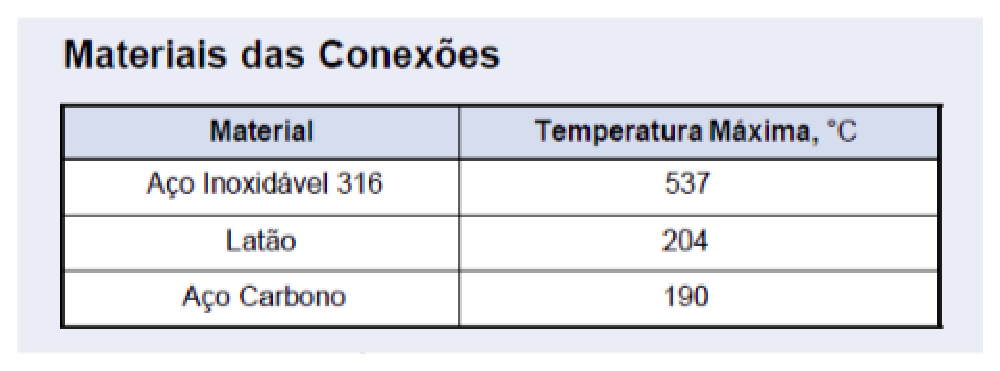
\includegraphics[scale=0.6, keepaspectratio=true]{figuras/temperaturaconectores.eps} 
   \caption{Projeto de travagem dos conectores SWAGELOK.}              
\end{figure}


Como diz Adriano Gonçalves (Resposável técnico da Swagelok), “Em relações comerciais, o material com o melhor custo e prazo de entrega é o latão, com seu preço final saindo por menos da metade do preço do aço inoxidável 316.”

Com todos os dados em mãos é possível determinar margem de segurança em relação a pressão (99\%) e temperatura (50\%).
Como informado anteriormente no relatório, temos três opções para implementação do sistema, que variam a quantidade de conectores. Em integração com o grupo de controle, discutimos quais conectores seriam precisos para a integração dos sistemas, após a discussão chegou-se ao consenso de quais conectores utilizar, independente da opção de implementação escolhida, o sistema precisa dos conectores listados abaixo: 

\begin{itemize}
\item 5 Redutores (2-Sensor de Fluxo, 2-Reservatório e 1-Sensor de Temperatura);
\end{itemize}

\begin{figure}[!htb]                                                               
   \centering                                                                      
   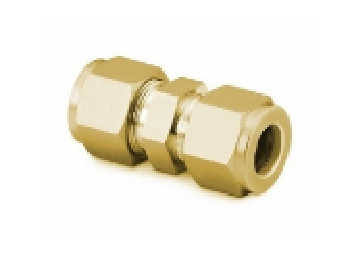
\includegraphics[scale=0.6, keepaspectratio=true]{figuras/peca1.eps} 
\end{figure}


\begin{itemize}
\item 2 T (Sensor de Pressão e de Temperatura);
\end{itemize}

\begin{figure}[!htb]                                                               
   \centering                                                                      
   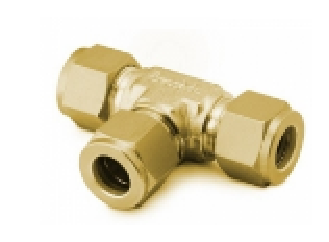
\includegraphics[scale=0.6, keepaspectratio=true]{figuras/peca2.eps} 
\end{figure}\begin{itemize}

\newpage
\item 2 Machos (Radiador);
\end{itemize}

\begin{figure}[!htb]                                                               
   \centering                                                                      
   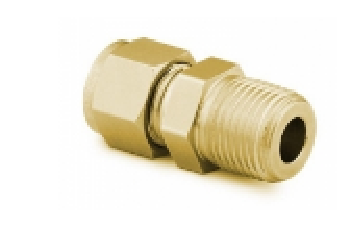
\includegraphics[scale=0.6, keepaspectratio=true]{figuras/peca3.eps} 
\end{figure}

A opção de implementação traz a variação da quantidade de cotovelos $90º$, tal variação é especificada na tabela abaixo:

\begin{table}[!h]
\centering
\begin{tabular}{|p{3cm}|p{5cm}|}
\hline
Opção & Número de cotovelos\\
\hline
1 & 4 \\ \hline
2 & 2 \\ \hline
3 & 2 \\
\hline
\end{tabular}
\caption{Variação de cotovelos}
\end{table}

\begin{figure}[!htb]                                                               
   \centering                                                                      
   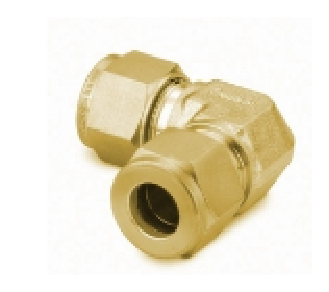
\includegraphics[scale=0.6, keepaspectratio=true]{figuras/peca4.eps} 
\end{figure}

\subsection{Reservatório}

Seguindo o requisito do professor sobre a utilização de materiais COTS, o reservatório escolhido é um reservatório de radiador automotivo, que se enquadra nas especificações necessárias, por ser fabricado em material de qualidade, com boa resistência a temperatura, além de contar com boa disponibilidade e baixo custo. 
A principal informação a se ter sobre o reservatório é sua capacidade, para o em questão a mesma é na faixa de 2 litros, tal capacidade é mais que necessária para o projeto, já que a partir de cálculos simples podemos determinar a quantidade de fluido em toda tubulação quando o sistema está hermeticamente fechado, uma condição primordial para a operação do sistema. Como informado anteriormente no relatório, temos três opções para implementação do sistema, que variam o comprimento da mangueira, modificando assim o volume de água no sistema.

\begin{table}[!h]
\centering
\begin{tabular}{|c|c|c|c|}
\hline
Opção & Comprimento da mangueira(m) & Quantidade de fluído na tubulação(ml) \\
\hline
1 & 6 & 42.40 \\ \hline
2 & 6.5 & 45.93 \\ \hline
3 & 7.8 & 54.40 \\
\hline
\end{tabular}
\end{table}

Com a ajuda da tabela acima podemos observar que a quantidade máxima de fluido presa na tubulação é 54,4 ml. O reservatório conta com a capacidade na faixa de 2 litros dando ao sistema uma margem de segurança na casa dos 90\%. 

O reservatório em questão é produzido a partir do PEAD (Polietileno de Alta Densidade) que conta densidade igual ou maior que $0,941 g/cm^3	$, um baixo nível de ramificações, com alta densidade e altas forças intermoleculares, trazendo características como:
\begin{itemize}
\item Resistente a altas temperaturas;
\item Alta resistência à tensão; compressão; tração;
\item Baixa densidade em comparação com metais e outros materiais;
\item Impermeável;
\item Inerte (ao conteúdo), baixa reatividade;
\item Atóxico
\item Pouca estabilidade dimensional 
\end{itemize}
O reservatório conta com dimensões gerais: 15 x 33 x 22 cm, e peso total (vazio): 355 gramas.


\begin{figure}[!htb]                                                               
   \centering                                                                      
   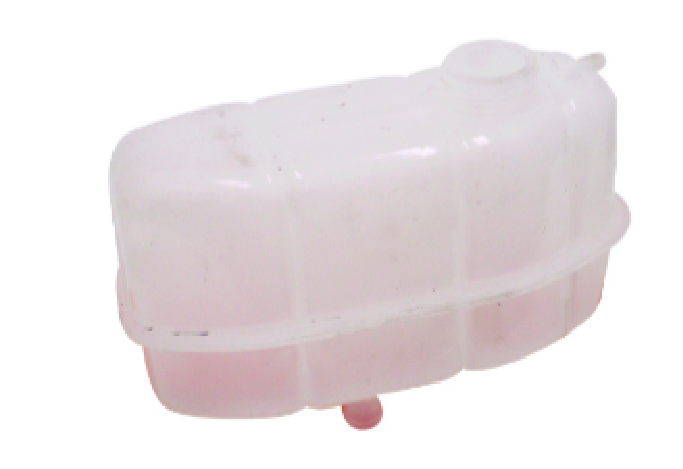
\includegraphics[scale=0.6, keepaspectratio=true]{figuras/reservatorio.eps} 
   \caption{Reservatório do radiador}
\end{figure}

\subsection{Riscos da estrutura}

Tendo  isso em vista, foram realizadas análises de riscos envolvendo 3 partes do projeto, sendo estas: riscos do sistema de bombeamento, riscos do sistema de arrefecimento e riscos na tubulação e reservatório.
Como medida de prevenção geral, antes do teste principal todo o sistema de refrigeração, bombeamento e tubulação serão testados previamente para, caso problemas sejam detectados, possam ser fixados sem prejuizos financeiros ou estruturais.

\subsubsection{Riscos do sistema de bombeamento}

Como parte principal de todo o sistema de refrigeração, a bomba deve ter um grau de confiabilidade muito alto pois, caso ela pare, o sensor chegará a uma temperatura onde os dados coletados são imprecisos e o teste será descartado.
Como medida de prevenção, duas bombas serão utilizadas para, caso uma venha a falhar, o teste possa continuar. A bomba A funcionará inicialmente enquanto a B está desligada. Em caso de mal funcionamento da A, a B será ligada e o teste continuará sem interrupções. 

\begin{figure}[!htb]                                                               
   \centering                                                                      
   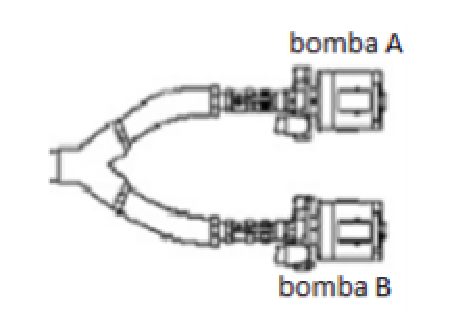
\includegraphics[scale=0.6, keepaspectratio=true]{figuras/conexaobombas.eps} 
   \caption{Representação do sistema das bombas}
\end{figure}

Para que haja a troca da bomba durante o teste, duas válvulas serão utilizadas. Uma para a saída das bombas, esta sendo livre, e uma para a entrada da bomba, esta com um servo motor. A primeira válvula ficará fechada para a bomba B e, caso a bomba A falhe, será ativado o fluxo na bomba B e a própria impulsão da bomba abrirá a válvula a fechando para a bomba A. Já na entrada do sistema, haverá um servo motor conectado ao sistema de monitoramento geral. Quando for indicada a falha na bomba, o servo se ativará e fechará o fluxo para a bomba A, abrindo, simultaneamente, para a bomba B.

Como prevenção, serão utilizados fuzíveis para proteção elétrica e bombas com menos de 30.000 horas de uso, a fim de aumentar a confiabilidade do sistema.

\subsubsection{Riscos do sistema de arrefecimento}
Assim como o bombeamento d'água, a refrigeração tem um grau de importância alto. Falhas também são imperdoáveis. 
Toda a água será refrigerada no radiador, porém o que pode vir a falhar são os coolers que o ventilam.  Como medida de prevenção serão utilizados 4 coolers (o dobro do que acompanha os radiadores). Dessa forma além da taxa de refrigeração aumentar, a chance de que todos os coolers venham a falhar é mínima. 
De qualquer forma, caso 3 ou mais coolers parem, o nível de refrigeração abaixará e o teste será desconsiderado por sobreaquecimento do sensor.

\subsubsection{Riscos da tubulação no reservatório}

Alguns dos riscos técnicos presentes no projeto, tem relação com a ocorrência de falha na tubulação do sistema e no reservatório de água. Esses riscos englobam o vazamento de água nas mangueiras, nas conexões entre os tubos ou no reservatório, e o rompimento da ligação entre os tubos e os conectores.
Para lidar com esses riscos, foram elaboradas 3 (três) medidas de prevenção e uma medida de contenção.


\subsubsection{Prevenção e contenção dos riscos estruturais}

Alguns dos riscos técnicos presentes no projeto, tem relação com a ocorrência de falha na tubulação do sistema e no reservatório de água. Esses riscos englobam o vazamento de água nas mangueiras, nas conexões entre os tubos ou no reservatório, e o rompimento da ligação entre os tubos e os conectores.

As medidas preventivas serão:

\begin{itemize}
\item O sistema de bombeamento de água funcionará abaixo da sua potência máxima. Isso proporciona ao sistema a garantia de que, na ocorrência de vazamentos, o fluxo líquido da água (fluxo de saída da bomba menos o fluxo de vazamento) seja constante durante o teste.
\item Para garantir que o sistema não possui vazamentos, será inicializado todo o sistema de bombeamento antes do teste, afim de averiguar, no reservatório, nas conexões e ao longo da mangueira, a integridade da tubulação.
\item Tendo em vista a possibilidade de vazamentos durante o teste do foguete, será utilizado um reservatório maior que o necessário, para garantir ao sistema o mínimo de água necessária para arrefecer o sensor 6061B.
\end{itemize}

A medida de conteção é delimitada abaixo:

\begin{itemize}
\item Caso o nível do reservatório diminua mais que o previsto durante o teste e atinja uma marca menor que 10\% da sua capacidade, o sistema será desligado e o teste desconsiderado.
\end{itemize}

\newpage

\subsection{Resultados pós-pesquisa para estruturas}

Ao levar em conta as pesquisas realizadas anteriormente, os seguintes materiais foram escolhidos para cada subsistema estrutural.

\begin{table}[htb]
\begin{tabular}{|p{3cm}|p{4cm}|p{3cm}|p{2cm}|p{3cm}|}
\hline
Subsistema & Modelo & Quantidade & Preço(R\$) & Orçamento(R\$) \\
\hline
Bomba & DC30QA-1230  & 2 & 33,48 & 66,96 \\ \hline
Radiador & Radiador de alumínio com conexões G $1/4$, 240 mm & 1 & 150,00 & 150,00\\ \hline
Cooler & Cooler FAN “CoolerMaster Sickleflow 12cm R4-SXDP-20FB-R1 & 4 & 35,18 & 140,72\\ \hline
Tubulação & Politetrafluoretileno (PTFE) & - & - & -\\ \hline
Conectores & Swagelok, Latão & - & -  & - \\ \hline
Reservatório & PEAD (Polietileno de Alta Densidade) de 15 x 33 x 22 cm & 1 & - & - \\ \hline
Válvulas & Válvula dupla de entrada de água - Lavadora Electrolux  & 2 & 45,00 & 90,00\\ \hline
\hline
\end{tabular}
\caption{Orçamento de materiais}
\end{table}

Com isso o orçamento total para a parte estrutural do projeto se dá em R\$ 447,68.
A montagem do sistema dos materiais será realizada de acordo com a figura descrita na seção de estrutura do sistema.